% !TeX root = ../../main.tex

Our re-statement of the TCC in terms of a surrounding sub-levelset of a function $f$ sets us up with most of the machinery we need to approximate its persistent homology.
However, because the TCC only confirms coverage of a \emph{superlevel} set $D\setminus B_\omega$, we cannot guarantee coverage of the entire domain.
% However, assuming we have a sample that satisfies the TCC we do not know that we cover the entire domain, but only the \emph{super-levelset} $D\setminus B_\omega$.
% As we would like to analyze the persistent homology of $f$ in a way that extends the TCC we will not approximate the persistence of this \emph{restriction} of $f$ using techniques from previous work~\cite{chazal09analysis}.
Indeed, we could compute the persistent homology of the \emph{restriction} of $f$ to the superlevel set we cover in the standard way~\cite{chazal09analysis}.% , or that of the super-levelset filtration down to $\omega$ using previous work~\cite{chazal09analysis}.
% As we would like to analyze the persistent homology of $f$ in a way that extends the TCC
Instead, we will approximate the persistent homology of the sublevel set filtration \emph{relative to} the sublevel set $B_\omega$.
That is, we will compute the relative persistent homology of $f$ with respect to a \emph{static} sublevel set $B_\omega$.

\begin{figure}[htbp]
  \centering
  \begin{minipage}[b]{0.27\textwidth}
    
\includegraphics[trim=200 200 200 100, clip, width=\textwidth]{scripts/figures/surf/ass2_C_side.png}\\
    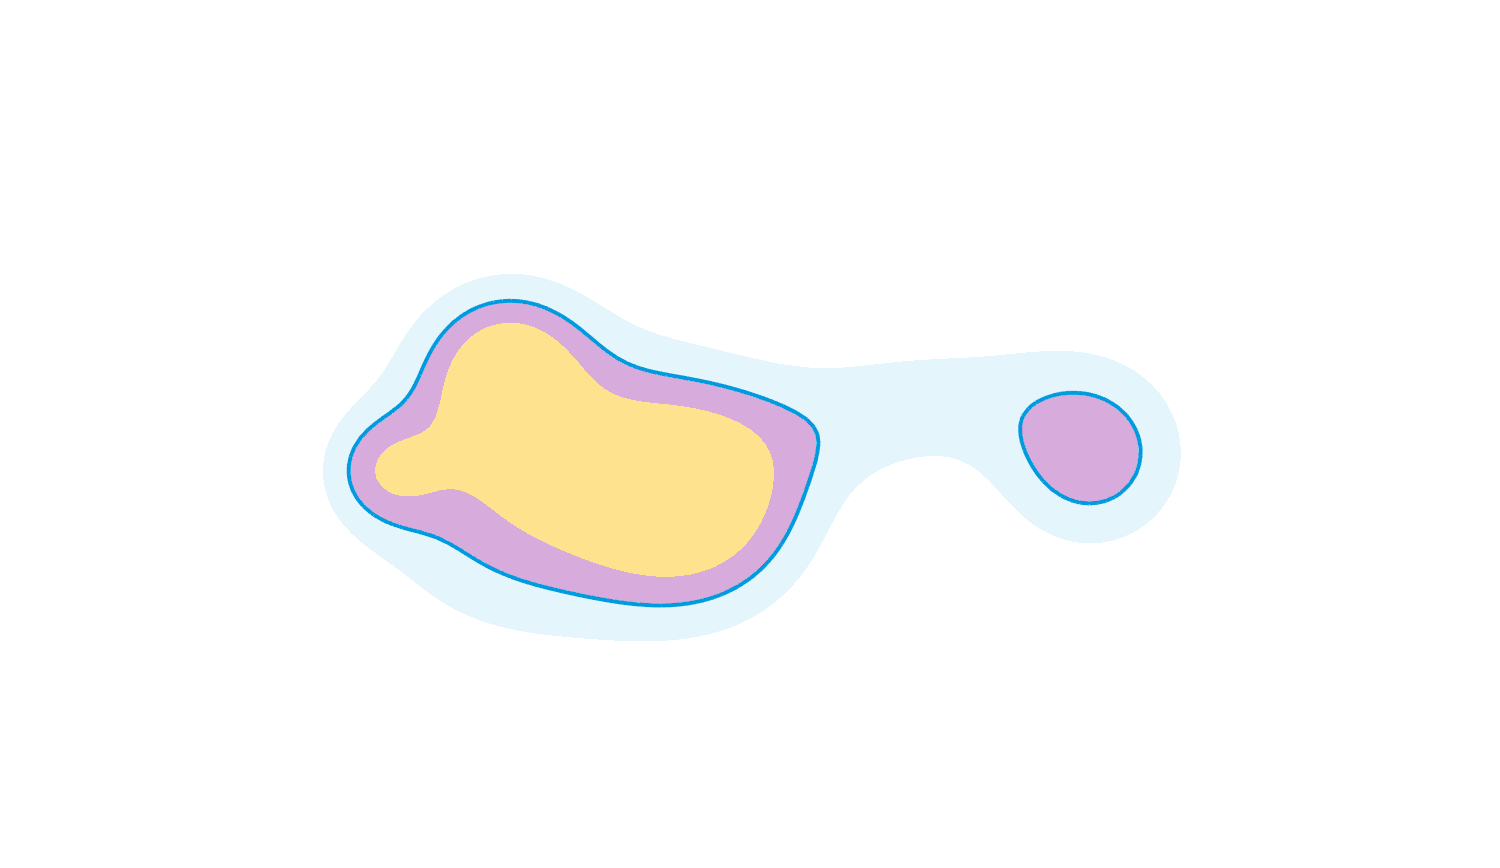
\includegraphics[trim=200 100 200 200, clip, width=\textwidth]{scripts/figures/surf/ass2_C_top.png}
  \end{minipage}
  \begin{minipage}[b]{0.7\textwidth}
    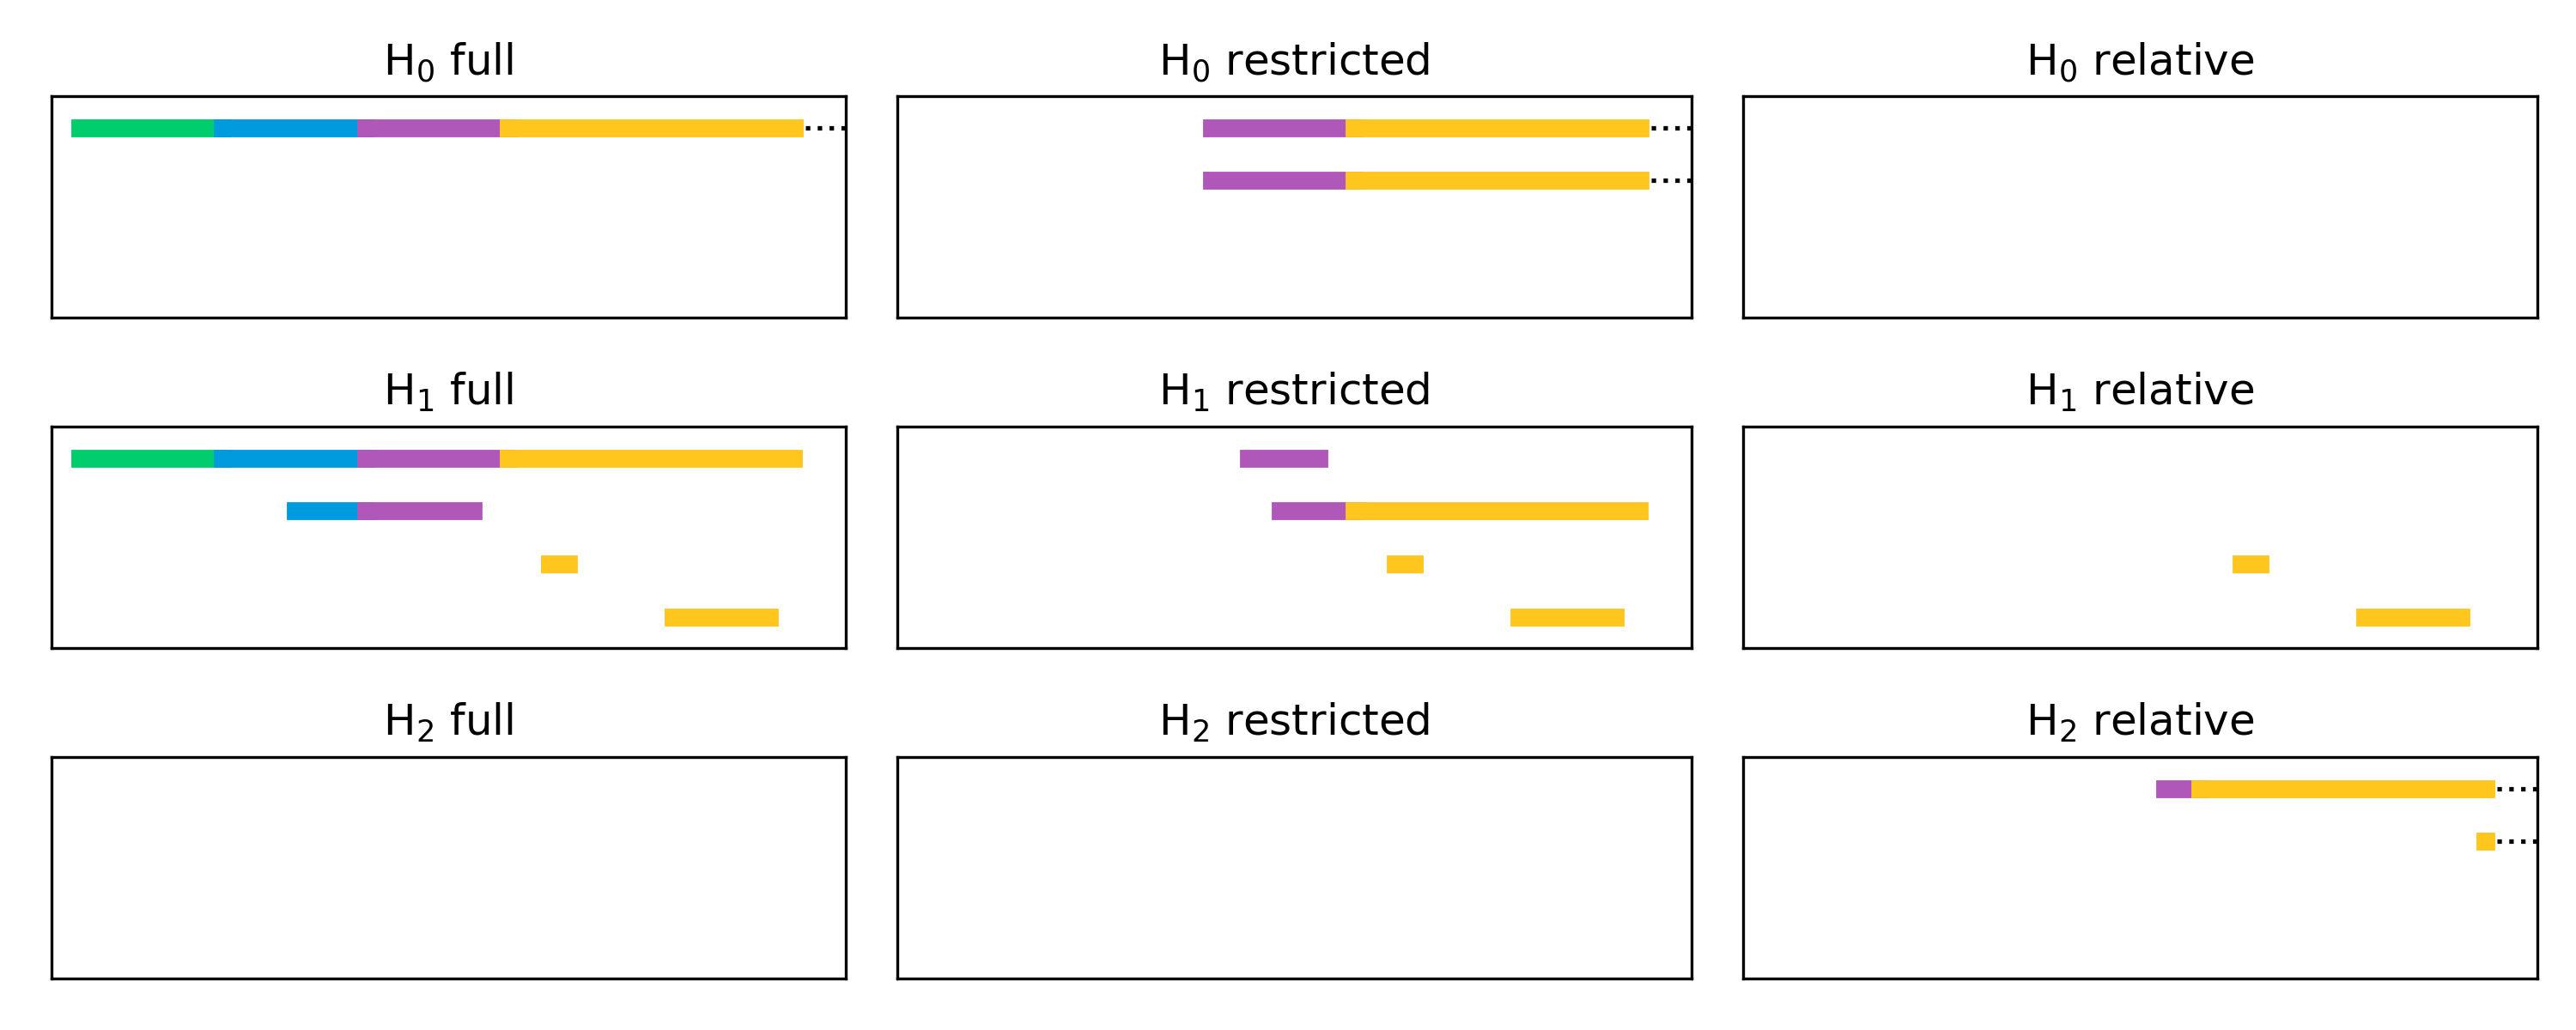
\includegraphics[width=\textwidth]{scripts/figures/barcodes/res_rel.png}
  \end{minipage}
  \caption{Full, restricted, and relative barcodes of the function (left).% on a $512\times 512$ grid.
    The restricted barcode is of the function restricted to the region above the blue line.
    The relative barcode is of the function relative to the blue sub-levelset below the blue line.}
    % We note that the additional features in restricted $\hom_0$ are artifacts of the restriction caused by the approximation.}

\end{figure}
% After providing an interleaving with an approximation by Vietoris-Rips complexes, as in the previous section, we will discuss how the resulting diagram is related to the \emph{truncated} diagram of $f$---the diagram of $f$ after $\omega$.
% We will then

% While persistent relative homology~\cite{todo} has been studied, interleaving relative modules requires interleaving pairs by pairs of shifted homomorphisms which, ideally, are induced by inclusions.
% However, taking the persistent homology relative to a \emph{static} sub-levelset $B_\omega$ without asserting that the corresponding approximation is homotopy equivalent.
% Moreover, the TCC only confirms coverage of a subset $D\setminus B_\omega$ so we cannot even assume we have coverage of some subset of $B_\omega$.

We will first introduce the notion of an extension which will provide us with maps on relative homology induced by inclusion via excision.
However, even then, a map that factors through our pair $(D, B_\omega)$ is not enough to prove an interleaving of persistence modules by inclusion directly.
To address this we impose conditions on sublevel sets near $B_\omega$ which generalize the assumptions made in the TCC on maps induced by the inclusions
\[ D\setminus B_{\omega+c(\delta+\zeta)}\hookrightarrow D\setminus B_\omega\hookrightarrow D\setminus B_{\omega-c(\delta+\zeta)}\]
on $0$-dimensional homology, to assumptions on maps induced by the corresponding inclusions
\[ B_{\omega-c(\delta+\zeta)}\hookrightarrow B_\omega\hookrightarrow B_{\omega+c(\delta+\zeta)}\]
on homology in all dimensions $k$.
To ease exposition we will introduce partial interleavings of image modules as a way to use these assumptions in our proof. % in the interleaving proof.
Section~\ref{sec:interleaving} will then set up notation and prove the interleaving in the geometric context introduced in section~\ref{sec:geo_tcc}.
% We therefore introduce image modules and partial interleaving as a way to use these assumptions to prove an interleaving.

% Section~\ref{sec:interleaving} will set up notation and prove the interleaving in the geometric context introduced in section~\ref{sec:geo_tcc}.
% We will then discuss how the resulting diagram is related to the \emph{truncated} diagram of $f$---the subdiagram of $f$ after $\omega$.
% Finally, we will compare this with the diagram of the function \emph{restricted} to the covered region, and show how approximations of the truncated diagram are better suited in certain cases.
